%!TEX root =  ../main.tex

\chapterimage{CMS_higgs-event} 
\mychapter{Regressions}{regression}
Many situations in science are about taking actual fuzzy numbers and attempting to
derive equations from them.    Sometimes these numbers are completely obvious,
practically screaming what kind of equation they come from.  On the other hand,
it can be deeply obscure and require enough care to regress from numerical
to algebraic information.  

But the consequences can be high.  Later generations may attempt to take your
equation and extrapolate well beyond the bounds you ever intended.  If you have
the wrong model, results can be disastrous, or at least, very upsetting (like the change
from Newtonian to Einsteinian physics).

\newpage
\chapterminitoc

%									13 - 1
\newpage
\invisiblesection{Graphical Patterns}
\subsection{Problems}
\noindent\makebox[\textwidth]{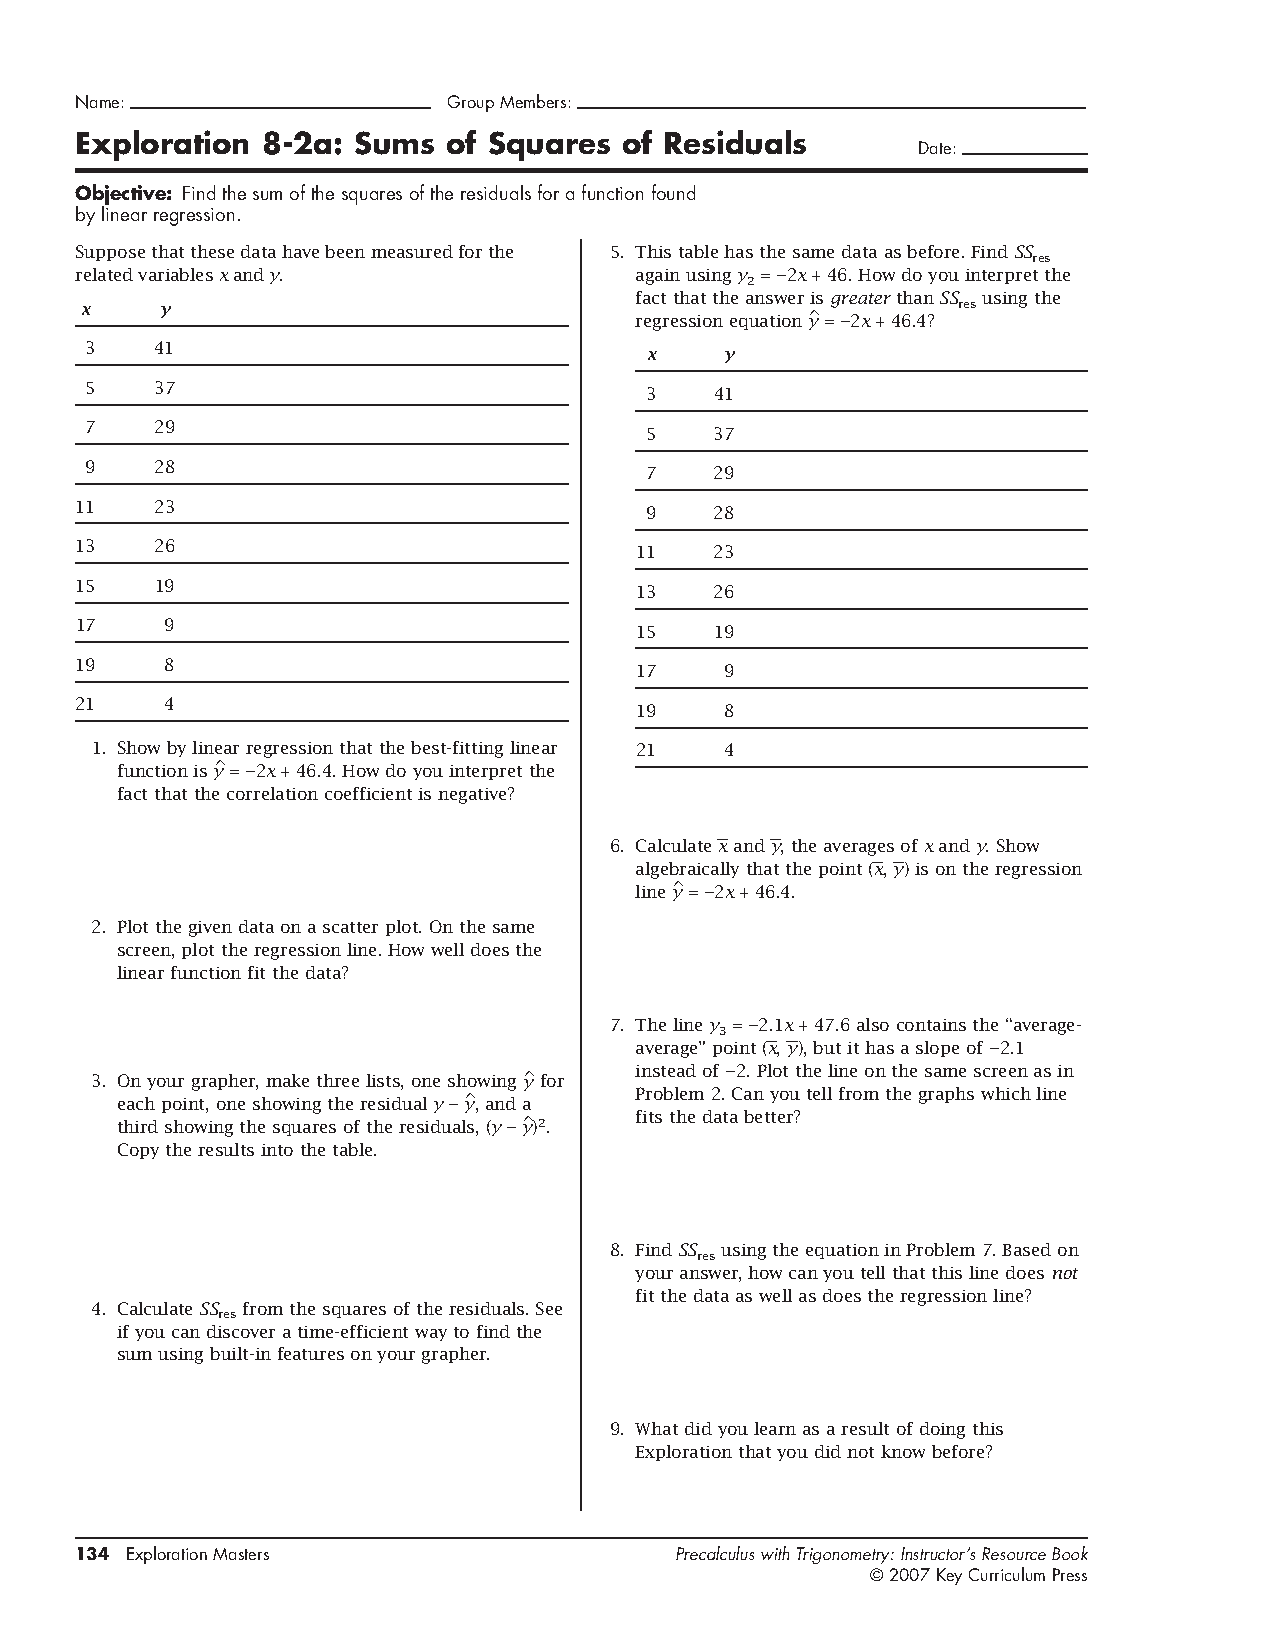
\includegraphics[width=\paperwidth]{ch13/1301p.pdf}}
\newpage
\subsection{Increasing/Decreasing}
\subsection{Concavity}
\subsection{Asymptotes}
\subsection{Origin Question}
\subsection{Repeating}
\subsection{End Behavior}
\newpage
\subsection{Exercises}

%									13 - 2
\newpage
\invisiblesection{Numerical Patterns}
\subsection{Problems}
\noindent\makebox[\textwidth]{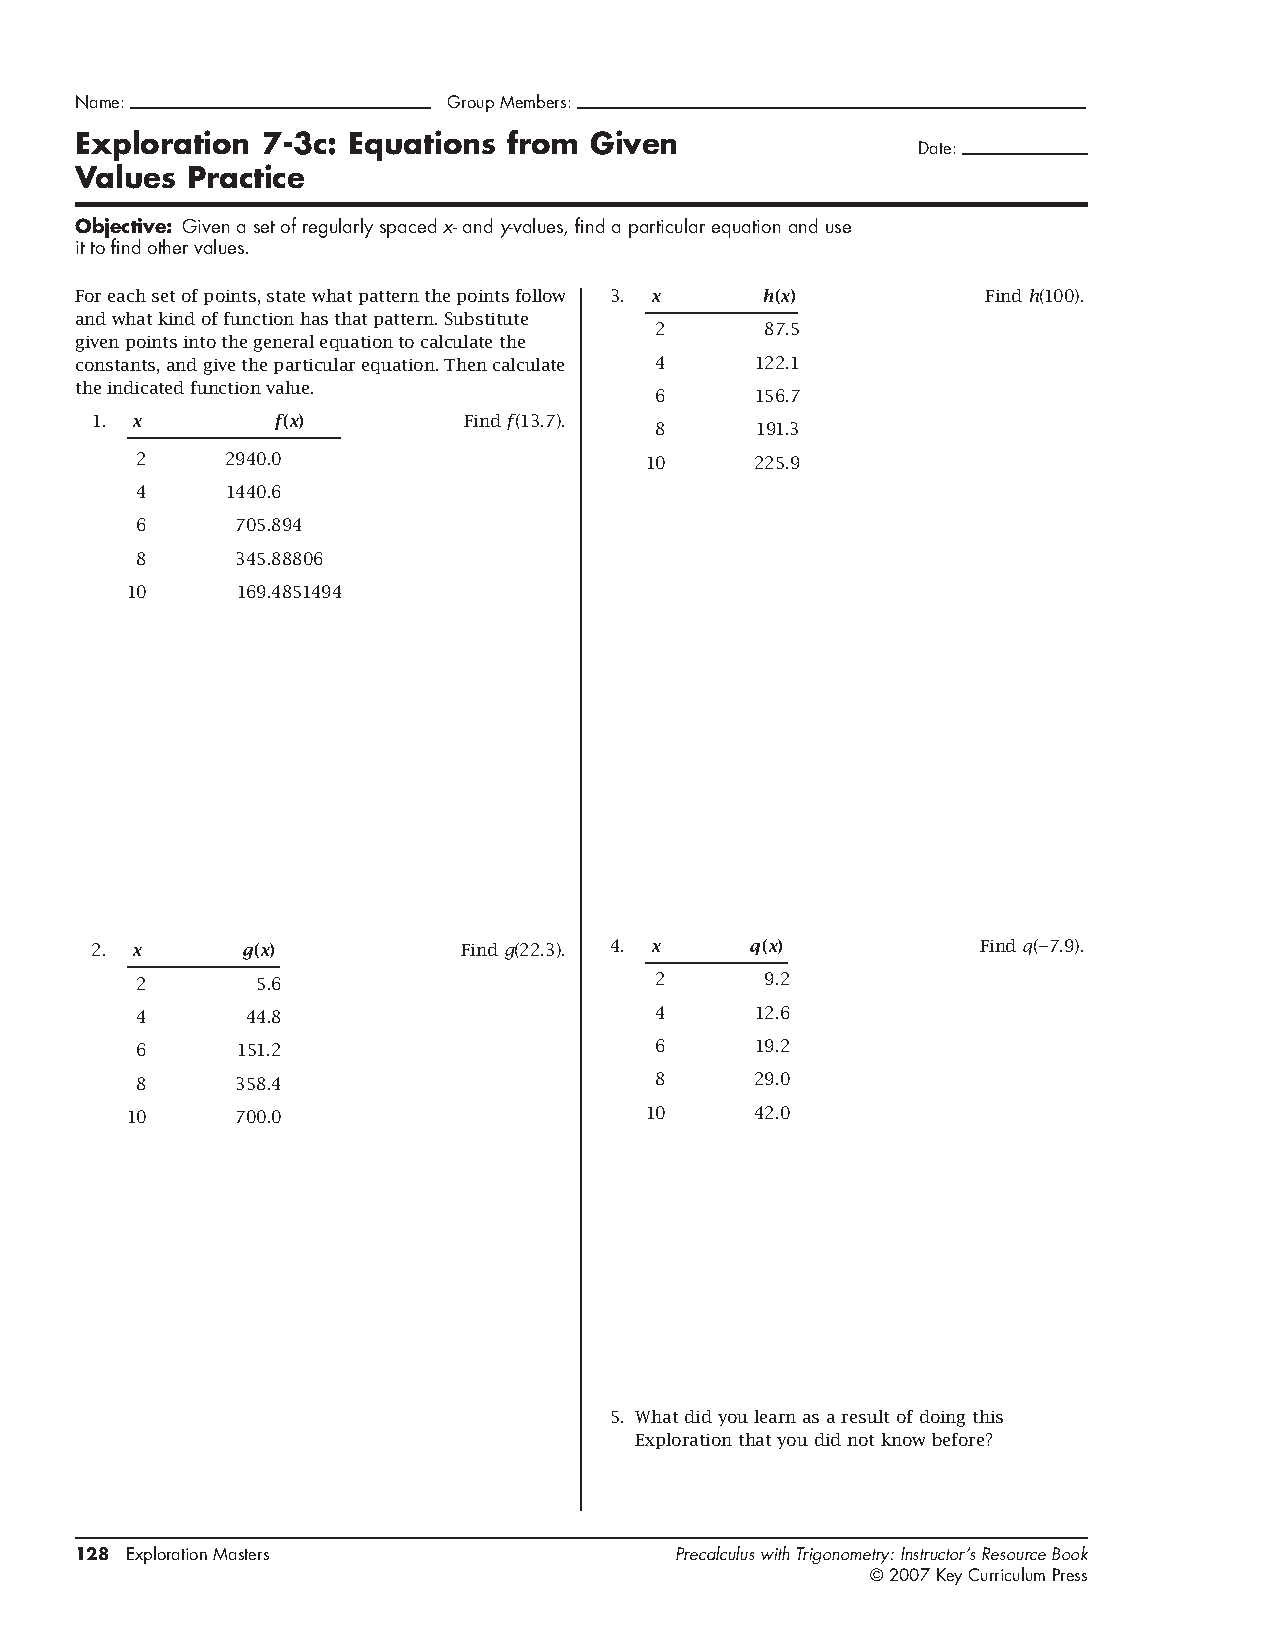
\includegraphics[width=\paperwidth]{ch13/1302p.pdf}}
\newpage
\subsection{Add-Add}
\subsection{Add-Multiply}
logs are multiply add
\subsection{Multiply-Multiply}
roots are divide divide
\subsection{Second Difference}
cubes are add third diff.

periodic the same data reoccurs at a constant interval
\newpage
\subsection{Exercises}

%									13 - 3
\newpage
\invisiblesection{Error}
\subsection{Problems}
\noindent\makebox[\textwidth]{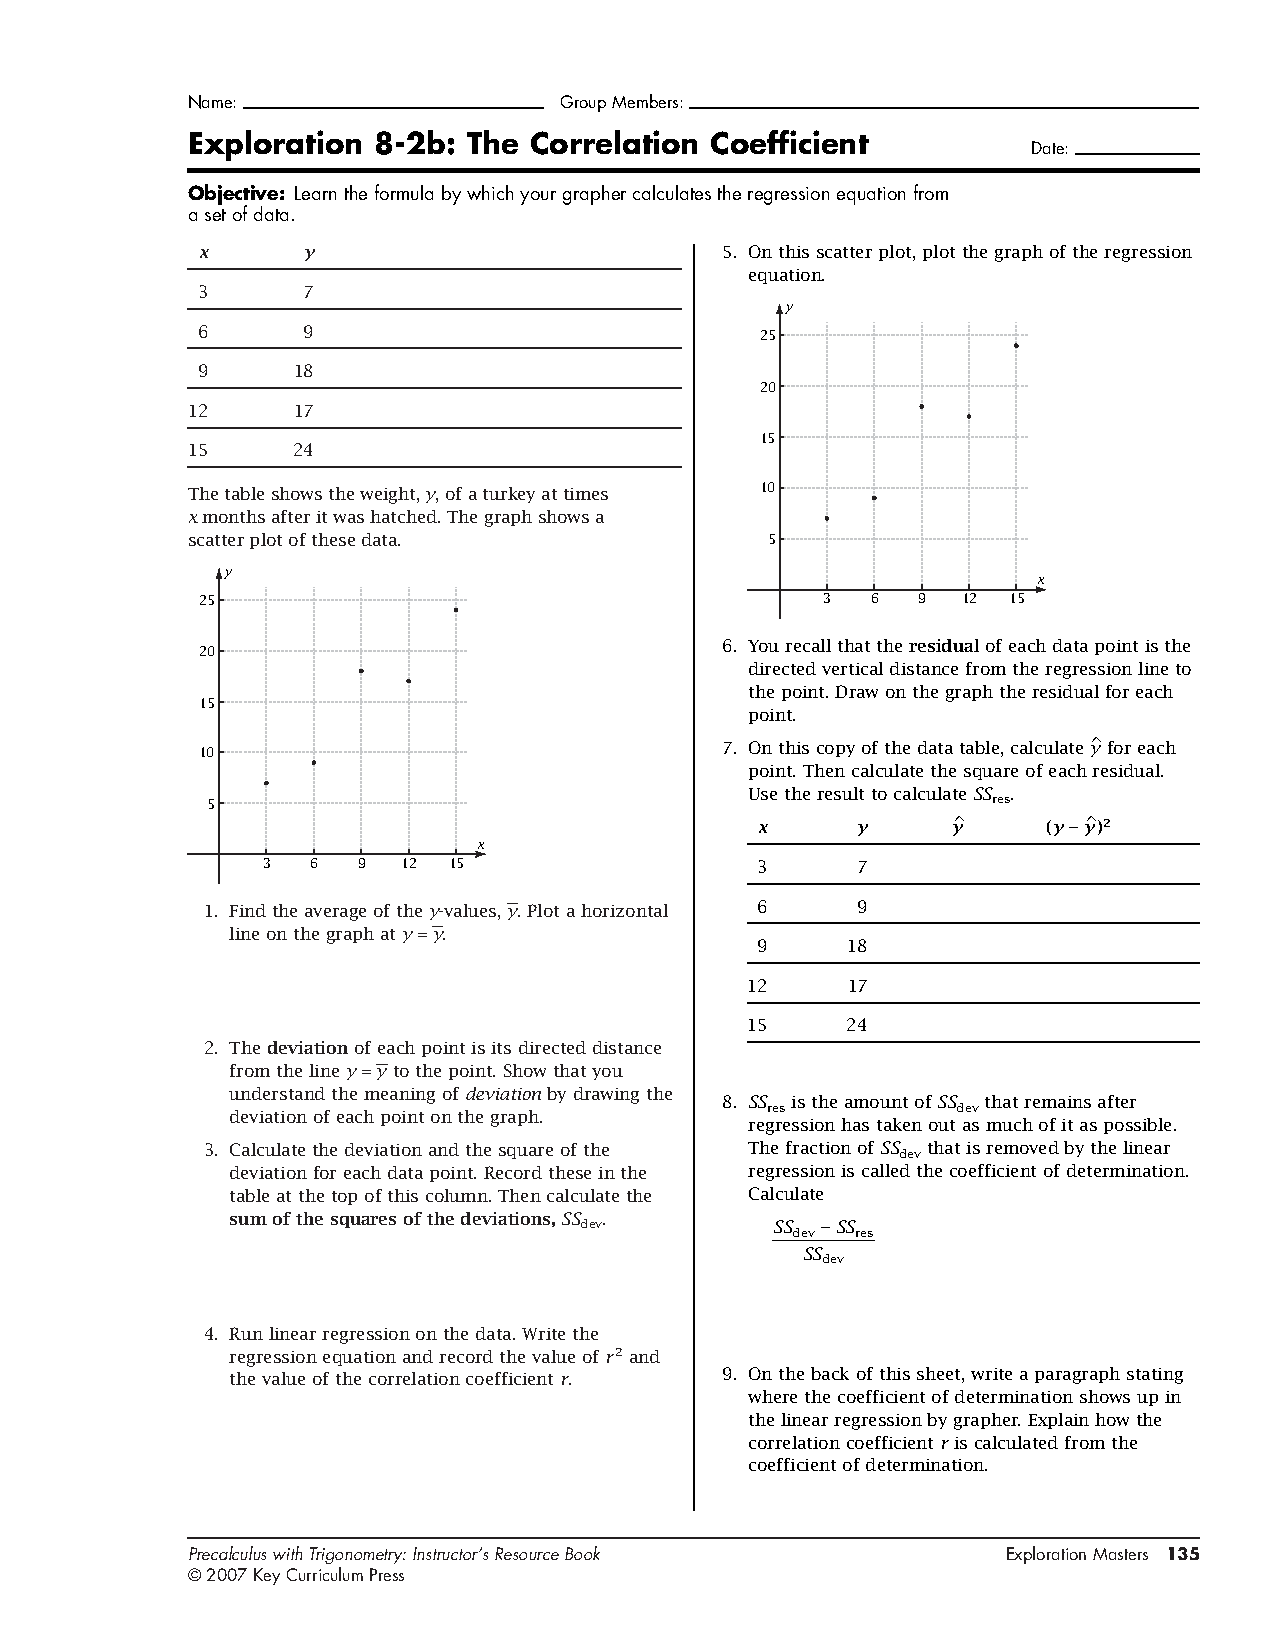
\includegraphics[width=\paperwidth]{ch13/1303p.pdf}}
\newpage
\subsection{SSres}
\subsection{SSdev}
\subsection{r vs $r^2$}
\newpage
\subsection{Exercises}

%									13 - 4
\newpage
\invisiblesection{Linearization}
\subsection{Problems}
\noindent\makebox[\textwidth]{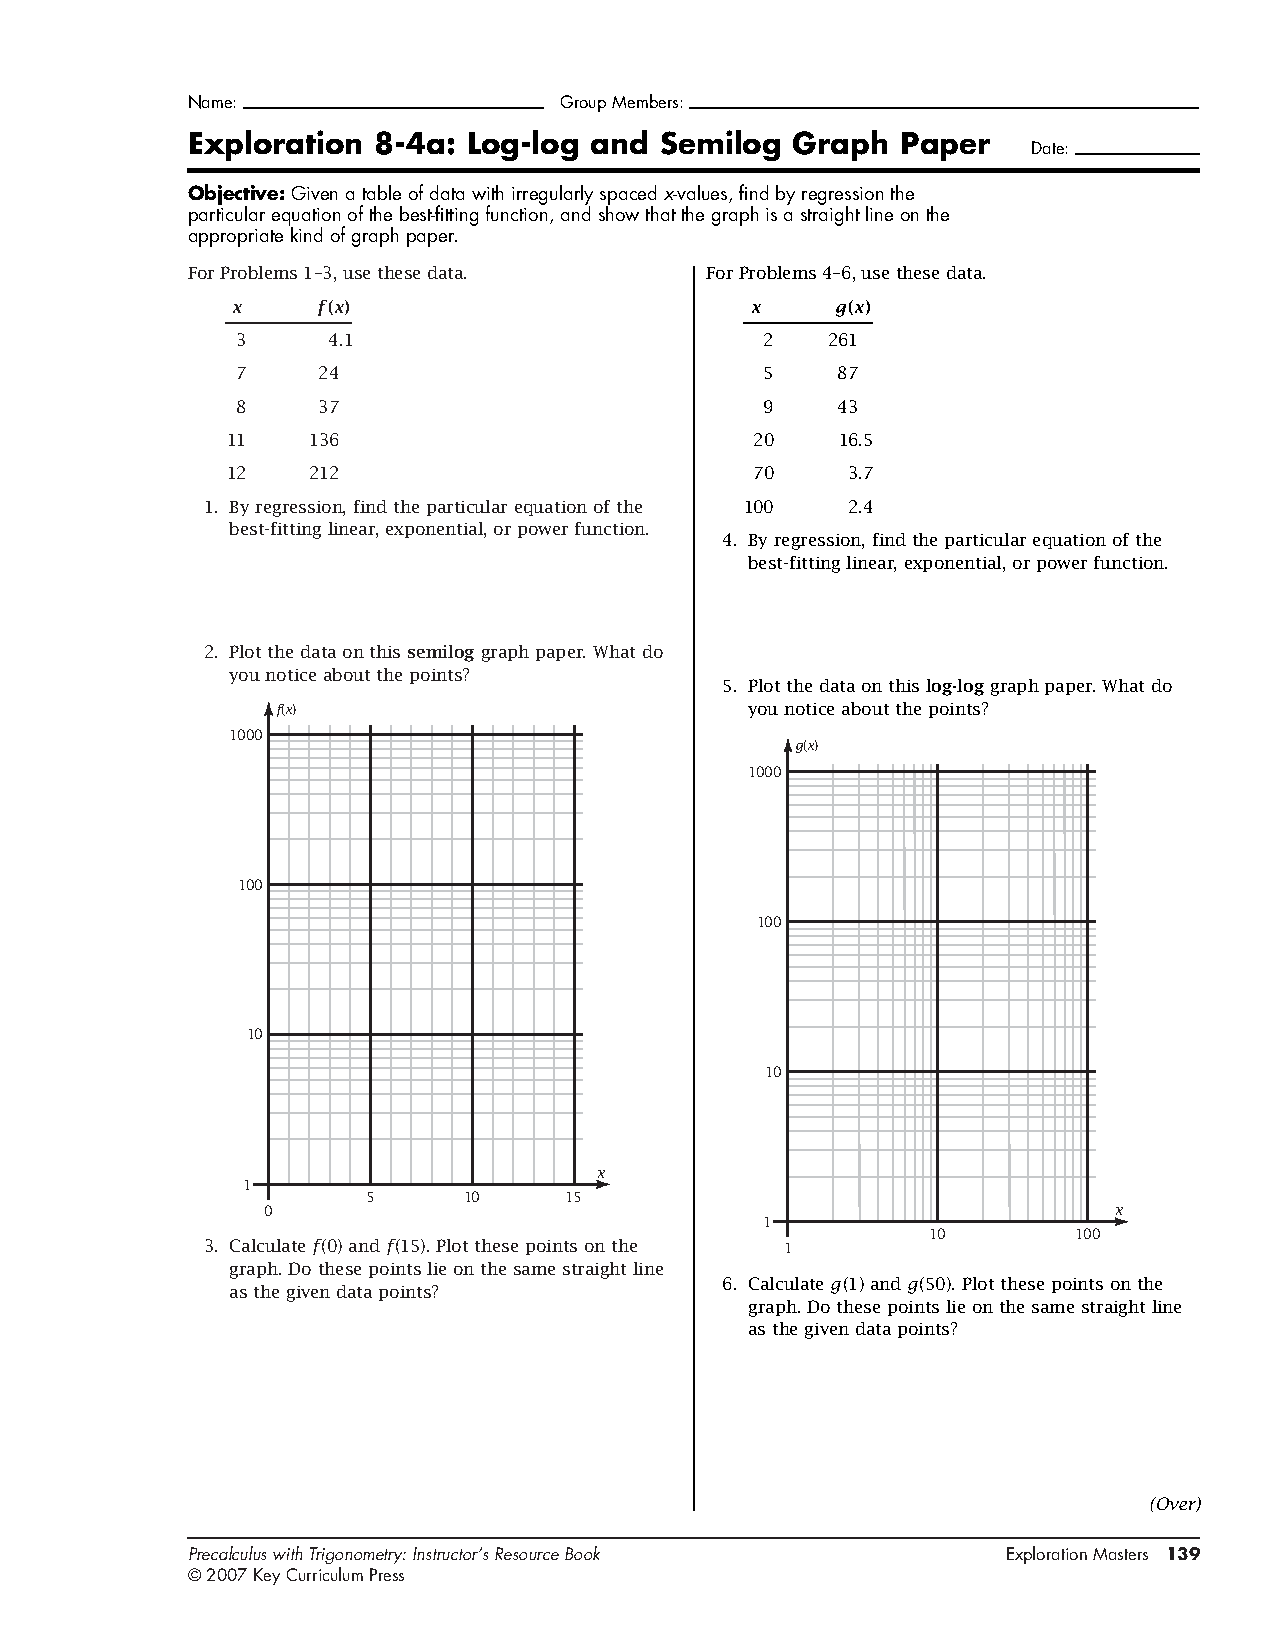
\includegraphics[width=\paperwidth]{ch13/1304p.pdf}}
\newpage
\subsection{Who gets the log?}
\subsubsection{Lin-Log Graphs}
\subsubsection{Log-Log Graphs}
\newpage
\subsection{Exercises}


%									13 - 5
\newpage
\invisiblesection{Differential Equations}
\subsection{Problems}
\noindent\makebox[\textwidth]{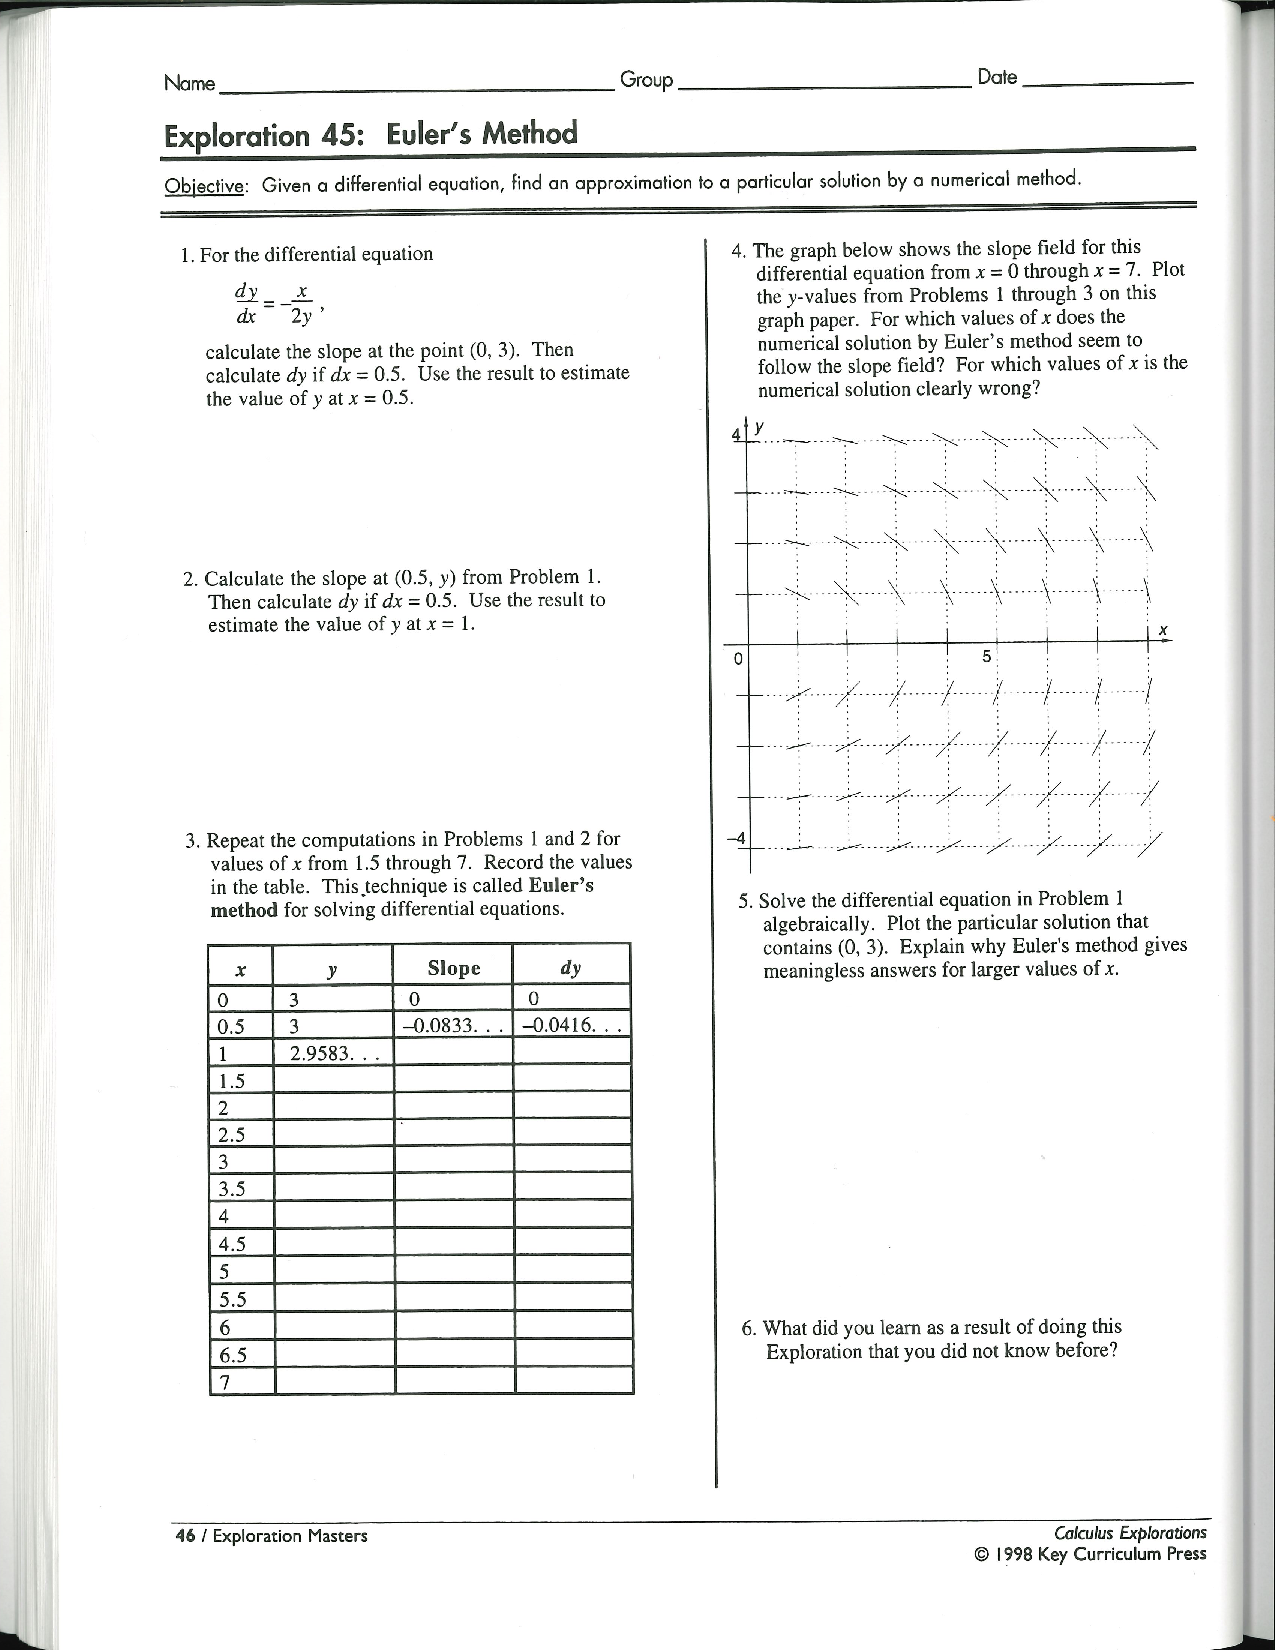
\includegraphics[width=\paperwidth]{ch13/1305p.pdf}}
\newpage
\subsection{Slope Fields}
\subsection{Euler's Method}
\subsection{Logistic Curves}
\newpage
\subsection{Exercises}


%									13 - 6
\newpage
\section{Review}
\subsection{Chapter Review}
\subsection{Chapter Test}